\documentclass[12pt,a4paper]{article}
\renewcommand{\baselinestretch}{1.05}
\usepackage[spanish]{babel}
%\usepackage[utf8]{inputenc}

\usepackage{amsmath,amsthm,verbatim,amssymb,amsfonts,amscd, graphicx}
\usepackage{graphicx}
\usepackage{caption}
\usepackage{subcaption}
\usepackage{tkz-fct}
\usetikzlibrary{babel}
\usepackage{pgfplots}
\usepackage{booktabs}
\usepackage{float}
\usepackage{enumitem}
\usepackage{forest}
\usepackage{hyperref}
\usepackage{ragged2e}

%Uso de la fuente Source Sans Pro

\usepackage[default]{sourcesanspro}
%\usepackage[T1]{fontenc}

%Controlar la partición de palabras.
\pretolerance=5000 
\tolerance=6000

%Simbolo de euro
\usepackage{eurosym} % para el euro


%Definición de monospace para codigo inline y paquete listings para código fuente.
\def\code#1{\texttt{#1}}
\usepackage{listingsutf8}
\lstset{
    %extendedchars=false,
    %inputencoding=utf8
}
\usepackage{color}
\definecolor{grisclarito}{gray}{0.95}

\lstdefinestyle{customc}{
  %belowcaptionskip=1\baselineskip,
  breaklines=true,
  frame=single,
  %xleftmargin=\parindent,
  language=C,
  showstringspaces=false,
  %basicstyle=\ttfamily,
  keywordstyle=\bfseries\color{green!40!black},
  commentstyle=\itshape\color{purple!40!black},
  identifierstyle=\color{blue},
  stringstyle=\color{orange},
  backgroundcolor=\color{grisclarito}
}

\hypersetup{
  colorlinks=true,
  linkcolor=black,
  urlcolor=blue
}

\setlength{\parindent}{0pt}
\topmargin0.0cm
\headheight0.0cm
\headsep0.0cm
\oddsidemargin0.0cm
\textheight23.0cm
\textwidth16.5cm
\footskip1.0cm

\renewcommand*\contentsname{Índice}

\begin{document}
\pgfplotsset{compat=1.16}
\begin{titlepage}
  \centering
  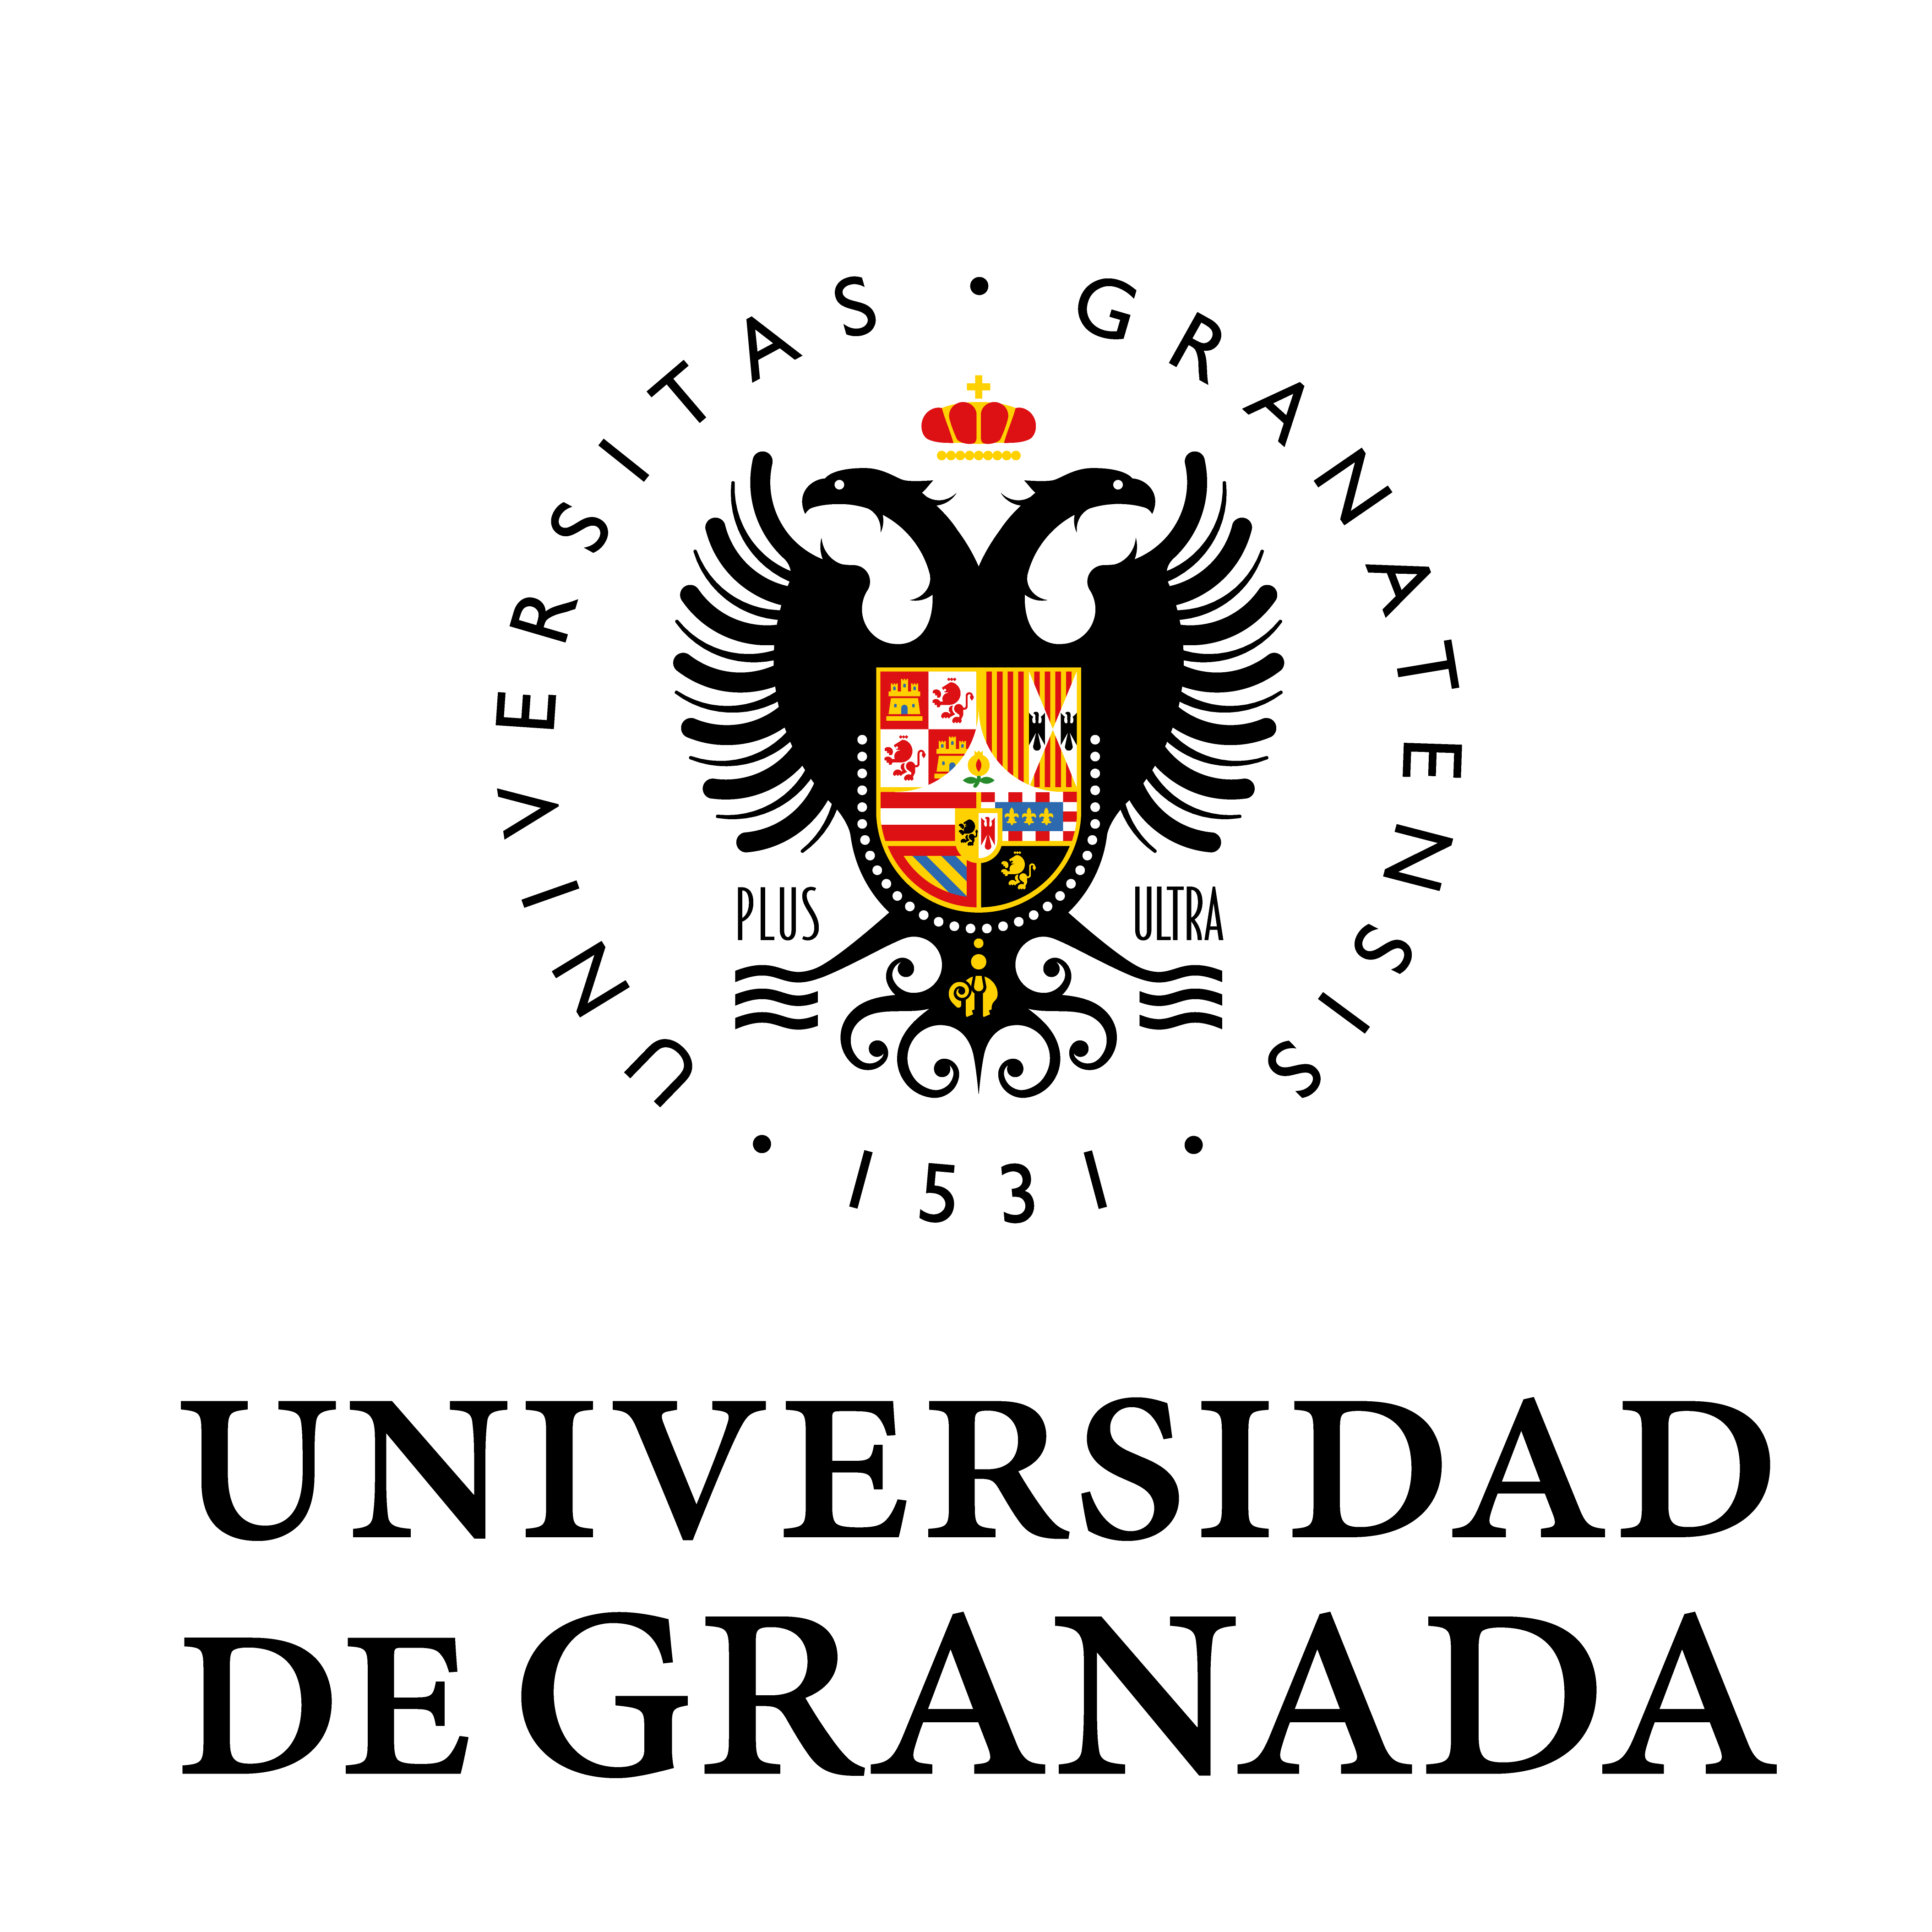
\includegraphics[width=0.6\textwidth]{ugr.png}\par\vspace{1cm}
  {\scshape\large Metodologías de desarrollo ágil \par} \vspace{1cm}
  {\huge\bfseries DSDM: Dynamic System Development Method \par}
  \vspace{0.4cm}
  {\large\itshape Un método iterativo y creciente\\}
  \vspace{0.6cm}
  {\large\itshape  Pedro Bonilla Nadal \\ David Infante Casas \\ Laura García Gómez \\ Antonio Martín Ruiz \\ Juan Ocaña Valenzuela  \par} \vspace{1.00cm}
  Curso 2019-2020 \\
  \vfill

  % Bottom of the page
  {\large \today\par}
\end{titlepage}

\tableofcontents
\newpage

\setlength{\parskip}{10pt}
\justify

\section{Introduccion}
El método de desarrollo de sistemas dinámicos (Dynamic Systems Development Method, DSDM) es un framework para el desarrollo de software de forma ágil creado en 1995 por lo que actualmente se conoce como el Consorcio DSDM. Determina fases, subfases y principios que permiten a equipos de desarrollo trabajar de forma eficiente. Fue una metodología muy popular durante los años 90 y comparte cualidades con otros métodos de desarrollo ágil como SCRUM o Programación Extrema. Es por esto que no es una metodología muy explotada a día de hoy, pues muchos equipos prefieren el uso de SCRUM. DSDM se divide en tres fases: preproyecto, ciclo de vida del proyecto y postproyecto. A su vez, el ciclo de vida se subdivide en cuatro fases, viabilidad, exploración, ingeniería y despliegue.

\begin{center}
 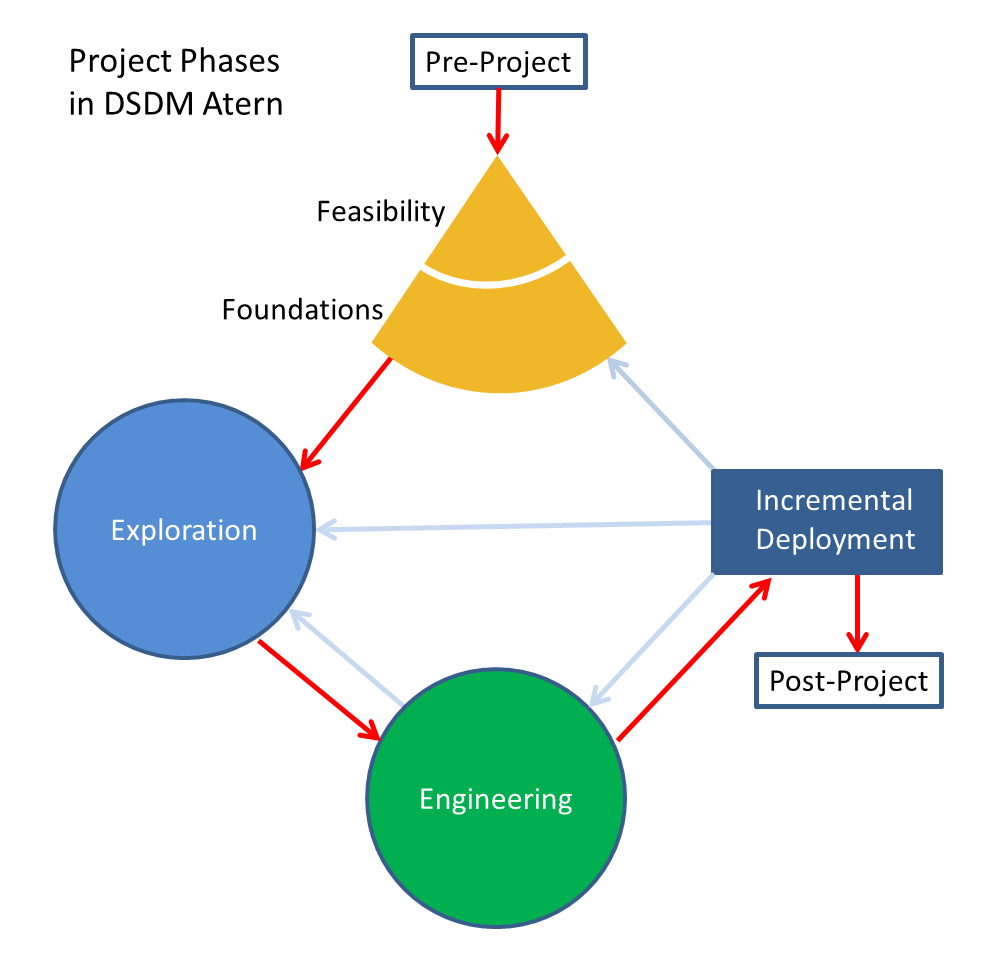
\includegraphics[width=0.6\textwidth]{DSDM_Phases.png}
\end{center}

DSDM es el método ágil más antiguo, lanzado en 1995 y es el único método ágil para centrarse en la gestión de proyectos ágiles. Arie van Bennekum representó a DSDM en el lanzamiento de Agile Alliance y su Agile Manifesto en 2001. DSDM ha operado principalmente en el ambiente corporativo donde demuestra consistentemente su habilidad para trabajar exitosamente dentro y complementar los procesos corporativos existentes. Practicando el desarrollo evolutivo, la última versión de DSDM (Atern) incorpora esas mejoras.


Algunas características de DSDM incluyen al usuario como componente activo durante el desarrollo, equipos bien preparados y lanzamiento de prototipos frecuente. También se usa la técnica <<Timeboxing>>, de la cual hablaremos más adelante, en la que se establecen intervalos en los que se liberarán los prototipos. Estos intervalos son muy similares a los sprints de SCRUM.



% Preproyecto: Es vital que el equipo de desarrollo satisfaga la mayoría de roles. Los principales son: - El patrocinador ejecutivo es alguien que actúa como el CEO de una empresa. - El rol de visionario lo lleva a cabo alguien responsable de la detección inicial de requisitos para comenzar el proyecto, el cual también actúa como product manager. - El usuario embajador es alguien con un gran conocimiento sobre el público objetivo y ofrece feedback al equipo de desarrollo. Se trata de un consultor externo. - El Project manager es responsable de que el proyecto se complete con éxito y el día a día del mismo. - Desarrolladores y testers.

%Ciclo de vida del proyecto: Primero se realiza un estudio de viabilidad y al acabar el estudio de negocio se determinan los requisitos funcionales y no funcionales, se diseña la arquitectura del software y el plan de desarrollo. Durante esta fase inicial los dos roles más importantes son los de Project Manager y CEO. Se detallan los costes y beneficios del desarrollo y se evaluan.
% Durante la segunda fase, los líderes de proyecto y el equipo de desarrollo trabajan junto con el usuario embajador para crear un prototipo funcional y asegurar su correcto desarrollo.
% En la tercera fase, los roles de visionario y patrocinador ejecutivo pierden valor. El proyecto se desarrolla en iteraciones y el consultor externo se involucra para asegurar que las necesidades de los usuarios estén cubiertas.
%En la última etapa, se presenta el sistema a los usuarios y se incorpora el feedback durante varias iteraciones.

\section{Fases del desarrollo}
Para explicar las fases de desarrollo, de entre las diversas variedades de DSDM, explicaremos en particular las del DSDM-Atern. Atern difiere de los enfoques ágiles más comunes en que abarca todo el ciclo de vida del proyecto y no sólo el desarrollo de software (donde prevalece Scrum). Incorpora disciplinas de gestión de proyectos y proporciona mecanismos para asegurar que los beneficios del proyecto sean claros, que la solución propuesta sea factible y que existan bases sólidas antes de que se inicie el trabajo detallado. .


\begin{itemize}
	\item P\underline{re-proyecto}: Inicio del proyecto, acordando los Términos de Referencia para el trabajo.
	\item \underline{Viabilidad}:
	Normalmente una fase corta para asegura cual es el valor del proyecto y resaltar su modelo de negocio.
	\item \underline{Fundaciones}: Fase clave para asegurar que el proyecto se entienda y defina lo suficientemente bien como para que el alcance se pueda basar en un alto nivel y los componentes y estándares tecnológicos se acuerden, antes de que comience la actividad de desarrollo.

\item \underline{Exploración}: Fase de desarrollo iterativo durante la cual los equipos amplían los requisitos de alto nivel para demostrar la funcionalidad.

\item \underline{Ingeniería}: Fase de desarrollo iterativo en la que la solución se diseña para que pueda desplegarse para su lanzamiento.

\item \underline{Despliegue}: Para cada incremento (conjunto de cuadros de tiempo) del proyecto se pone a disposición la solución.

 \item \underline{Post proyecto}: Evalúa los beneficios acumulados.

Las fases de exploracion y la fase de ingenieria normalmente se mezclan, dado que el método es flexible, permitiendo a los equipos que lo adapten para ser más adecuado a su situación. Como podemos ver estas fasen comprenden dentro de ellas 


\section{Principios}

\section{Roles}

\section{TimeBoxing}
La gestión de proyectos tradicional utiliza \emph{miletones} para acordar un asset a realizar para un proyecto determinado en un punto en el tiempo. Si bien los  \emph{miletones} funcionan lo suficientemente bien, TimeBoxing es una técnica mucho más poderosa para lograr el mismo resultado. Una TimeBox es un intervalo, normalmente no más largo de 6 semanas, donde un conjunto dado de tareas debe ser logrado. El motivo de la duración relativamente baja de las TimeBox es el hecho de que los seres humanos dan estimaciones mucho más precisas en el futuro cercano, con un pequeño conjunto de tareas.
En las estimaciones de un futuro lejano, en el que intervienen grandes conjuntos de tareas, se acaban produciendo grandes errores.\\

 Una TimeBox puede contener varias tareas, y al final de esta se ha de buscar entregar un producto. Los  \emph{miletones} también
sufren de tener un entregable fijo, mientras que los TimeBoxes están sujetas a cambios, ya que
se definen las tareas, no necesariamente el entregable, que puede cambiar si cambios de prioridades durante la iteración del TimeBox, lo que permite una respuesta rápida a
necesidades del negocio. En resumen: DSDM deja de lado la funcionalidad a favor de la entregar a tiempo. 

Podemos observar como característivas en el uso de timeboxing en combinación con las fases del proyecto DSDM:
\begin{enumerate}
	\item  Los Timeboxes pueden ser de diferente longitud.
	\item  Varias de las mismas fases de DSDM pueden ejecutarse inmediatamente después de una
la TimeBoxde la misma fase ha terminado.
\item Las TimeBoxesparalelas son posibles, incluso las TimeBoxescomplementarias son
permitido.
\item Diferentes fases de DSDM pueden ser realizadas en una TimeBoxal mismo tiempo.
tiempo.
\item Los Timeboxes pueden ser anidados.
\end{enumerate}


\end{itemize}



\section{Conclusiones}

{\color{red} \rule{\linewidth}{0.5mm} }
{\color{blue} TODO: hola, podemos añadir de la página https://www.methodsandtools.com/archive/dsdmatern.php cuales son los princpipiso, los roles y los productos.}\\
{\color{red} \rule{\linewidth}{0.5mm} }

%Bibliographic references
\begin{thebibliography}{9}

\bibitem{pickpocketing} Dynamic Systems Development Method (DSDM)
\\\texttt{http://www.students.science.uu.nl/~slegt001/me/final\_5767202\_Slegten.pdf}
\bibitem{pickpocketing2}Dynamic System Development Method
\\\texttt{https://files.ifi.uzh.ch/rerg/arvo/courses/seminar\_ws03/14\_Voigt\_DSMD\_Ausa-\\rbeitung.pdf}
\bibitem{pickpocketing3}New Directions on Agile Methods:A Comparative Analysis
\\\texttt{http://secure.com.sg/courses/ICT353/Session\_Collateral/TOP\_03\_ART\_06\_ARTI-\\CLE\_ABRAHAMSSON\_New\_Directions\_Agile\_Methods.pdf}

\bibitem{pickpocketing4}Agile software developmentmethods.
\\\texttt{http://www.vtt.fi/inf/pdf/publications/2002/P478.pdf}


\bibitem{pickpocketing5}Introduction to DSDM Atern
\\\texttt{https://www.methodsandtools.com/archive/dsdmatern.php}
\end{thebibliography}

\end{document}
